\section{Диффузия легирующей примеси}

Приконтактные области выполняют роль резервуаров электронов. Концентрация донорной примеси в них увеличивается ступенчато. Ближайшая к активной области приконтактная область имеет уровень легирования $N_{D}^{r} = 2*10^{23}$м$^{-3}$, размер данной области $r = 20$ монослоев (см рис.\ref{fig:RTHSResearch}). Следующая за приконтактной область имеет степень легирования выше на порядок, например, $N_{D}^{r+} = 2.5*10^{24}$м$^{-3}$.

\begin{figure}[h!]
	\centering
	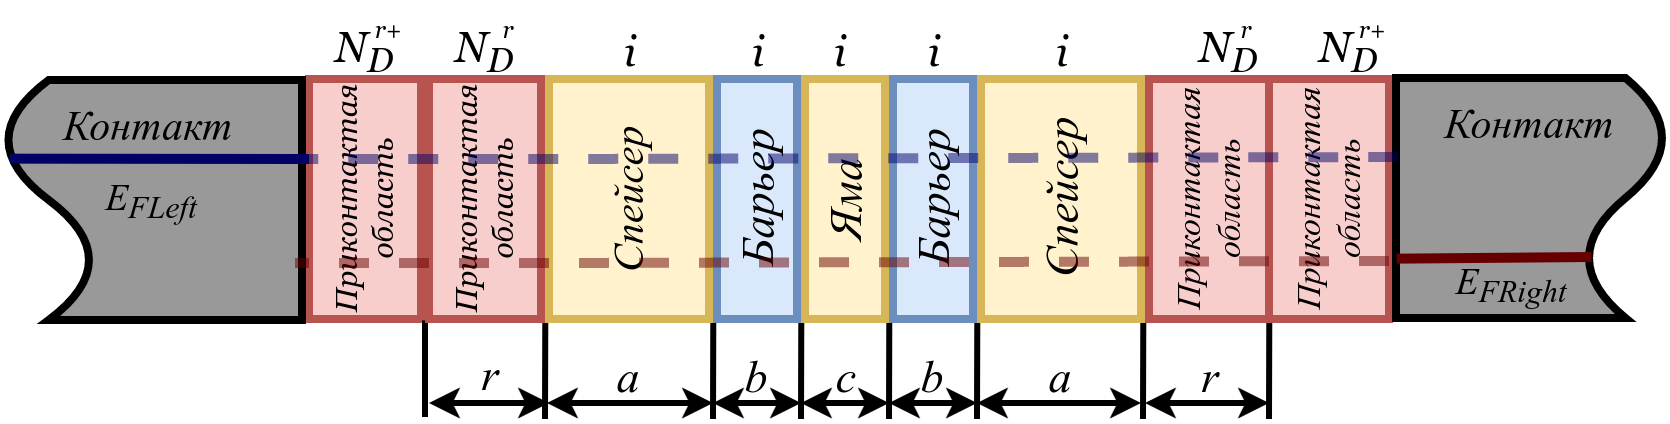
\includegraphics[width=.95\linewidth]{RTHSResearch}
	\caption{Модель исследуемой РТГС} 
	\label{fig:RTHSResearch}
\end{figure}

\begin{figure}[h!]
	\centering
	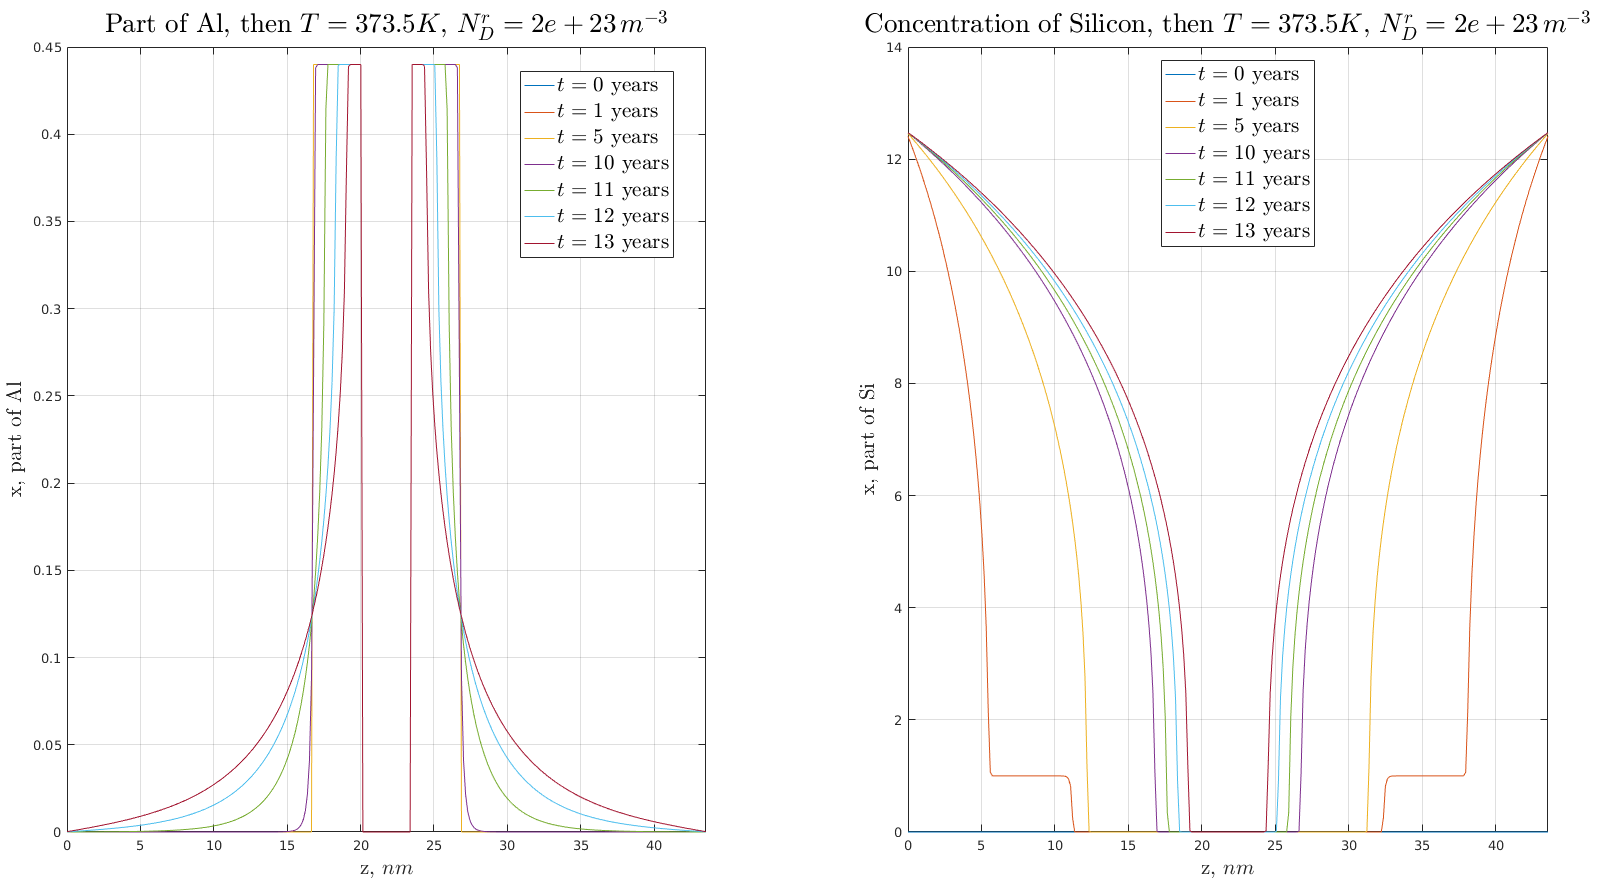
\includegraphics[width=.9\linewidth]{DSi100}
	\caption{Деградация при $T = 100^{\circ}$C c учетом приконтактных областей}
	\label{fig:DSi100}
\end{figure}



Из результатов термической деградации видно, что $Si$ и сильно легированной приконтактной области доходит только через $10$ лет, а следовательно ВАХ РТГС за этот срок меняется незначительно, что было показано ранее. Результаты получены с помощью лист.\ref{lst:DSi} и лист.\ref{lst:DSiDiff}.